\chapter{Validation Results}

This chapter reports the final 2026-04-17 validation results rather than an intermediate checkpoint. All scoped suites now have named rerun records, the combined coverage export is archived on disk, and the inherited WR2 usability findings are now closed by the final rerun-backed evidence pack rather than carried as open blockers.

\section{Execution Summary}

\begin{table}[H]
\centering
\small
\begin{tabular}{llllll}
\toprule
\wcell{1.8cm}{\textbf{Date}} & \wcell{1.3cm}{\textbf{Mode}} & \wcell{4.7cm}{\textbf{Scope}} & \wcell{1.3cm}{\textbf{Total}} & \wcell{1.3cm}{\textbf{Passed}} & \wcell{1.5cm}{\textbf{Status}} \\
\midrule
\wcell{1.8cm}{2026-04-17} & \wcell{1.3cm}{EditMode} & \wcell{4.7cm}{Consolidated rerun of all EditMode suites on the mirrored coverage workspace} & \wcell{1.3cm}{57} & \wcell{1.3cm}{57} & \wcell{1.5cm}{Verified} \\
\wcell{1.8cm}{2026-04-17} & \wcell{1.3cm}{PlayMode} & \wcell{4.7cm}{Coverage-backed smoke rerun for the battle start path} & \wcell{1.3cm}{1} & \wcell{1.3cm}{1} & \wcell{1.5cm}{Verified} \\
\wcell{1.8cm}{2026-04-17} & \wcell{1.3cm}{Coverage export} & \wcell{4.7cm}{Combined EditMode + PlayMode report generation and archive writeback} & \wcell{1.3cm}{58} & \wcell{1.3cm}{58} & \wcell{1.5cm}{Archived} \\
\bottomrule
\end{tabular}
\caption{Final execution summary used by the validation report.}
\label{tab:execution-summary}
\end{table}

\begin{table}[H]
\centering
\small
\begin{tabular}{lll}
\toprule
\wcell{2.8cm}{\textbf{Execution measure}} & \wcell{1.8cm}{\textbf{Value}} & \wcell{6.1cm}{\textbf{Interpretation}} \\
\midrule
\wcell{2.8cm}{Total suite files} & \wcell{1.8cm}{`11`} & \wcell{6.1cm}{The scoped suite consists of `10` EditMode files plus `1` PlayMode smoke file.} \\
\wcell{2.8cm}{Total test methods} & \wcell{1.8cm}{`58`} & \wcell{6.1cm}{The current suite is large enough to support both dense appendix tables and quantitative reporting.} \\
\wcell{2.8cm}{Verified by named rerun} & \wcell{1.8cm}{`58`} & \wcell{6.1cm}{Every authored test method is now backed by an archived rerun record.} \\
\wcell{2.8cm}{Directly targeted runtime classes} & \wcell{1.8cm}{`10`} & \wcell{6.1cm}{Every scoped runtime target in the battle slice has at least one direct suite file.} \\
\wcell{2.8cm}{Smoke / integration paths} & \wcell{1.8cm}{`1`} & \wcell{6.1cm}{The battle bootstrap and first playable turn are covered by an end-to-end PlayMode checkpoint.} \\
\bottomrule
\end{tabular}
\caption{Execution position after the final reruns.}
\label{tab:execution-position}
\end{table}

\section{Coverage and Traceability Results}

\begin{table}[H]
\centering
\small
\begin{tabular}{lll}
\toprule
\wcell{2.8cm}{\textbf{Coverage metric}} & \wcell{1.8cm}{\textbf{Value}} & \wcell{6.1cm}{\textbf{Evidence meaning}} \\
\midrule
\wcell{2.8cm}{Runtime classes in report} & \wcell{1.8cm}{`11`} & \wcell{6.1cm}{The archived coverage report spans all runtime classes cited in the validation chapter.} \\
\wcell{2.8cm}{Covered lines} & \wcell{1.8cm}{`868`} & \wcell{6.1cm}{Taken from the archived multi-report coverage summary.} \\
\wcell{2.8cm}{Coverable lines} & \wcell{1.8cm}{`1169`} & \wcell{6.1cm}{Used as the denominator for the line-coverage claim.} \\
\wcell{2.8cm}{Line coverage} & \wcell{1.8cm}{`74.2\%`} & \wcell{6.1cm}{The report now has archived quantitative coverage evidence rather than package-only tooling claims.} \\
\wcell{2.8cm}{Covered methods} & \wcell{1.8cm}{`146`} & \wcell{6.1cm}{Shows that the suite closes most method-level behaviour in the scoped battle slice.} \\
\wcell{2.8cm}{Total methods} & \wcell{1.8cm}{`158`} & \wcell{6.1cm}{Method totals come directly from the archived coverage summary.} \\
\wcell{2.8cm}{Method coverage} & \wcell{1.8cm}{`92.4\%`} & \wcell{6.1cm}{Method coverage is materially stronger than the line aggregate, which is expected for UI-heavy scripts.} \\
\bottomrule
\end{tabular}
\caption{Archived coverage totals.}
\label{tab:coverage-totals}
\end{table}

\begin{figure}[H]
\centering
\begin{tikzpicture}
\begin{axis}[
    ybar,
    bar width=7pt,
    ymin=0,
    ymax=105,
    ylabel={Line coverage (\%)},
    symbolic x coords={BattleUI,CardButtonView,CardData,CardResolver,DeckManager,EnemyAI,GameRoot,GridManager,TileView,TurnManager,UnitController},
    xtick=data,
    xticklabel style={rotate=40,anchor=east,font=\scriptsize},
    nodes near coords,
    nodes near coords align={vertical},
    every node near coord/.append style={font=\tiny},
    width=0.96\textwidth,
    height=0.38\textheight,
    enlarge x limits=0.02,
    legend style={at={(0.5,1.08)},anchor=south,legend columns=2,font=\scriptsize}
]
\addplot[fill=orange!60] coordinates {(BattleUI,56.2)};
\addplot[fill=blue!45] coordinates {
    (CardButtonView,100)
    (CardData,95.6)
    (CardResolver,77.7)
    (DeckManager,100)
    (EnemyAI,100)
    (GameRoot,93.1)
    (GridManager,85.9)
    (TileView,93.3)
    (TurnManager,80.1)
    (UnitController,97.2)
};
\legend{Lowest coverage target,Other runtime classes}
\end{axis}
\end{tikzpicture}
\caption{Class-level line coverage from the archived report. `BattleUI` remains the lowest-covered runtime class, but the final clean rerun lifted it to `56.2\%`, above the report target line and backed by direct tests plus the PlayMode smoke path.}
\label{fig:class-line-coverage}
\end{figure}

\begin{table}[H]
\centering
\small
\begin{tabular}{lll}
\toprule
\wcell{2.5cm}{\textbf{Coverage evidence item}} & \wcell{2.0cm}{\textbf{Status}} & \wcell{6.4cm}{\textbf{Reason it is report-ready}} \\
\midrule
\wcell{2.5cm}{Requirements coverage matrix} & \wcell{2.0cm}{Archived} & \wcell{6.4cm}{All `10/10` scoped requirements now map to rerun-backed suites.} \\
\wcell{2.5cm}{Module/class coverage matrix} & \wcell{2.0cm}{Archived} & \wcell{6.4cm}{Every targeted runtime class now has a direct verified suite file.} \\
\wcell{2.5cm}{Execution summary table} & \wcell{2.0cm}{Archived} & \wcell{6.4cm}{The final EditMode rerun, PlayMode smoke rerun, and coverage export are all named records on disk.} \\
\wcell{2.5cm}{Line-coverage chart} & \wcell{2.0cm}{Archived} & \wcell{6.4cm}{The chart is derived from the archived 2026-04-17 coverage report rather than draft estimates.} \\
\wcell{2.5cm}{Representative test case appendix} & \wcell{2.0cm}{Archived} & \wcell{6.4cm}{The appendix now references only final verified suite labels.} \\
\bottomrule
\end{tabular}
\caption{Evidence readiness for the final report.}
\label{tab:evidence-readiness}
\end{table}

\section{Defect Summary}

\begin{table}[H]
\centering
\small
\begin{tabular}{lllll}
\toprule
\wcell{1.7cm}{\textbf{ID}} & \wcell{2.0cm}{\textbf{Area}} & \wcell{1.4cm}{\textbf{Severity}} & \wcell{4.8cm}{\textbf{Finding}} & \wcell{1.8cm}{\textbf{Status}} \\
\midrule
\wcell{1.7cm}{WR2-BUG-01} & \wcell{2.0cm}{Onboarding feedback} & \wcell{1.4cm}{Medium} & \wcell{4.8cm}{New-player guidance around the required unit-before-card order was previously too easy to miss.} & \wcell{1.8cm}{Fixed and verified} \\
\wcell{1.7cm}{WR2-BUG-02} & \wcell{2.0cm}{Enemy turn readability} & \wcell{1.4cm}{Medium} & \wcell{4.8cm}{Enemy actions were functionally correct, but the phase summary previously lacked enough emphasis.} & \wcell{1.8cm}{Fixed and verified} \\
\wcell{1.7cm}{WR2-BUG-03} & \wcell{2.0cm}{Battle-end handling} & \wcell{1.4cm}{High} & \wcell{4.8cm}{The battle loop previously risked continuing after elimination.} & \wcell{1.8cm}{Fixed and verified} \\
\wcell{1.7cm}{WR3-BUG-01} & \wcell{2.0cm}{Test execution pipeline} & \wcell{1.4cm}{Medium} & \wcell{4.8cm}{Early live-editor discovery exposed only part of the authored suite, creating a truth gap between inventory and rerun evidence.} & \wcell{1.8cm}{Fixed and verified} \\
\wcell{1.7cm}{WR3-BUG-02} & \wcell{2.0cm}{Coverage evidence gap} & \wcell{1.4cm}{Low} & \wcell{4.8cm}{Code Coverage was installed before the first archived export existed.} & \wcell{1.8cm}{Fixed and verified} \\
\bottomrule
\end{tabular}
\caption{Final defect summary.}
\label{tab:defect-summary}
\end{table}

\begin{table}[H]
\centering
\small
\begin{tabular}{llll}
\toprule
\wcell{1.6cm}{\textbf{ID}} & \wcell{3.4cm}{\textbf{Probable root cause}} & \wcell{3.4cm}{\textbf{Fix or mitigation already applied}} & \wcell{3.1cm}{\textbf{Prevention / next action}} \\
\midrule
\wcell{1.6cm}{WR2-BUG-01} & \wcell{3.4cm}{The prototype relied on weak onboarding affordances around the unit-before-card rule.} & \wcell{3.4cm}{Prompt wording and next-step messaging were strengthened, and the final `BattleUI` rerun verified the new flow.} & \wcell{3.1cm}{Keep the current prompt flow as a regression-backed behaviour and reretest after any wording or highlight change.} \\
\wcell{1.6cm}{WR2-BUG-02} & \wcell{3.4cm}{Enemy-phase feedback was functionally correct but visually understated.} & \wcell{3.4cm}{Enemy summaries and related `BattleUI` / `TurnManager` message paths were strengthened and verified in the final rerun.} & \wcell{3.1cm}{Rerun the summary/message checks after any later wording, log, or transition-layout change.} \\
\wcell{1.6cm}{WR2-BUG-03} & \wcell{3.4cm}{End-state logic was previously too weakly locked.} & \wcell{3.4cm}{`TurnManagerTests` verified the battle-end fix and the consolidated rerun confirmed it remained stable.} & \wcell{3.1cm}{Keep this suite as a permanent regression gate in future reruns.} \\
\wcell{1.6cm}{WR3-BUG-01} & \wcell{3.4cm}{The editor refresh and discovery state initially did not match the full authored inventory.} & \wcell{3.4cm}{Missing test metadata was corrected and the final rerun upgraded the suite to fully verified status.} & \wcell{3.1cm}{Use named rerun records rather than discovery-only editor visibility for future truth claims.} \\
\wcell{1.6cm}{WR3-BUG-02} & \wcell{3.4cm}{The coverage tool was not part of the original prototype workflow.} & \wcell{3.4cm}{The package was installed, batchmode coverage export was scripted, and the final archive was written under `coverage/2026-04-17/`.} & \wcell{3.1cm}{Refresh the same export path whenever WR3 evidence is extended later.} \\
\bottomrule
\end{tabular}
\caption{Root cause, mitigation, and prevention view for the final defect register.}
\label{tab:defect-root-cause}
\end{table}

The validation result is therefore stable rather than provisional. The report now has a rerun-backed suite, an archived quantitative coverage layer, and a defect register in which the inherited WR2 issues and the tooling blockers are all closed with named evidence.
